%%!TEX root = main.Rnw
\documentclass[english, 11pt]{article}
\usepackage{haziq_article}
\usepackage{knitr}
\begin{document}
%\listoftodos[To-do list]

%%%%%%%%%%%%%%%%%%%%%%%%%%%%%%%%%%%%%%%%%%%%%%%%%%%%%%%%%%%%%%%%%%%%%%%%%%%%%%%%
%%% USEFUL MACROS %%%%%%%%%%%%%%%%%%%%%%%%%%%%%%%%%%%%%%%%%%%%%%%%%%%%%%%%%%%%%%
%%%%%%%%%%%%%%%%%%%%%%%%%%%%%%%%%%%%%%%%%%%%%%%%%%%%%%%%%%%%%%%%%%%%%%%%%%%%%%%%
\newcommand{\Hlam}{\bH_\lambda}
\newcommand{\Vy}{\bV_y}
\newcommand{\liky}{(2\pi\psi)^{-n/2}\exp\left[-\frac{\Vert \by - }{2} \right]}





\section{Introduction}
\label{sec:intro}

Typically, I-prior models are estimated via maximum marginal likelihood using an EM algorithm. 
This is the preferred method because it is a stable way of obtaining the ML estimates due to the specific structure of the marginal covariance matrix of the responses. 
Note that once the random effects $\bw$ are marginalised out, we are in fact interested in estimating a \emph{structured covariance matrix} which depends on the scale parameters $\blambda$ and precision $\psi$, which can be a bit tricky. 
The \pkg{iprior} package implements this stable EM algorithm that ensures the components of the marginal log-likelihood value (either the log-determinant or the covariance matrix inverse) does not ``blow up'' when the precision parameter $\psi$ gets either too large or too small. 
For some data sets, numerical issues can indeed happen due to this, but it has been noticed that the EM algorithm would generally be able to handle such cases much better, than say, a direct maximisation of the marginal log-likelihood.


One would be forgiven to expect I-prior modelling to be enshrined in a fully Bayesian paradigm, instead of frequentists approaches of maximising likelihoods.
To be fair, the EM algorithm has a Bayesian flavour to it, in that it provides maximum a posteriori (MAP) estimates under improper priors $f(\blambda,\psi) \propto \text{const.}$, i.e. a uniform distribution over the entire support of the parameters. 
Further, the EM algorithm does result in a posterior distribution over the latent variables, though the use of this posterior is restricted to only obtaining the Empirical Bayes estimates of the random effects (that is, plugging in the ML estimates into the posterior mean function).
A connection between the EM algorithm and variational Bayesian methods have also been noted by \citet[p. 337]{gelman2014bayesian} and \cite{neal1998view}.


Nevertheless, the EM algorithm might leave many Bayesians unsatisfied, especially in view of a modelling approach whose name has the word ``I-prior'' in it. 
Critiques of MAP estimation argue that this is not very representative of Bayesian methods, because the result is merely a point estimate, whereas Bayesian methods should yield a distribution from which inference is done (e.g. posterior mean, median and credible intervals).
Some would even argue that ``expectations are the only things that make sense'' in Bayesian inference \citep{betancourt2017conceptual}.
See also \url{http://twiecki.github.io/blog/2017/02/08/bayesian-hierchical-non-centered/}.
This is the motivation behind a fully Bayesian estimation of I-prior models.


To proceed, we would need to assume some prior distributions on the parameters of interest, namely $\blambda$ and  $\psi$. 
The choice of priors is partly driven by the ease of manipulating the posterior. 
Often, as is the case with random effects models, the go-to methods for computing the posteriors are by way of some Markov Chain Monte Carlo (MCMC) method, rather than an explicit derivation of the posterior density of the parameters.
Regardless, choosing conjugate priors that leads to recognisable posteriors, then this would computationally benefit MCMC methods such as Gibbs sampling.
Gibbs sampling using \pkg{JAGS} has been a popular choice for Bayesian inference. 
However, we will see later on that for our I-prior model, problems with autocorrelation are evident from the MCMC diagnostics, which in turn affects inference.


We turn to another MCMC sampler in Hamiltonian Monte Carlo (HMC).
HMC is a novel application of Hamiltonian dynamics to explore the posterior state space of our parameters.
HMC is implemented in the \pkg{Stan} software, and the user does not require any knowledge of Hamiltonian dynamics to operate it. 
Although the HMC literature is pretty involved, \pkg{Stan} is able to determine automatically the correct tuning parameters for the sampler to work efficiently.
One particularly attractive property of HMC is that there is no computational advantage to providing conjugate priors. 
This then frees us to use priors which are appropriate for reasons other than computational efficiency.


In particular, we could also include the Hurst coefficient as part of the MCMC sampler, to be estimated from a posterior distribution given some prior. 
This is certainly a nice feature, and something that is very difficult to do properly in a frequentist setting (i.e. obtaining the ML estimate Hurst coefficient). 
Note that there are optimisation methods to find the MLE of the Hurst coefficient; one simple method is a golden section search in the interval of valid Hurst coefficient values with the aim of minimising the profiled deviance of the marginal model \citep{jamil2017}.
Perhaps more sophisticated optimisation techniques can be used, but there is an appeal of simplicity and coherence to including the Hurst coefficient in the MCMC sampler.


In Section \ref{sec:gibbs}, we introduce the Bayesian I-prior model with an aim to implement Gibbs sampling. 
We will also see that Gibbs sampling produces terrible posterior samples, and \hltodo[Don't really know why yet]{we give some reasons as to why this might be}.
We then turn to HMC in Section \ref{sec:hmc}, starting with a brief introduction and then implementing the HMC sampler for the I-prior model in \pkg{Stan}.
A simulated example to estimate an I-prior model which uses the fractional Brownian motion kernel (FBM) is given.
A real-world example is also looked at, but some difficulties arise there.
Finally, the merits Bayesian method and the MLE method are discussed in the final section.



\section{Bayesian estimation using Gibbs sampling}
\label{sec:gibbs}

\subsection{The model}

The I-prior model is
\begin{align}\label{eq:iprior}
\begin{gathered}
	\by = \balpha + \Hlam\bw + \bepsilon \\
	\bw \sim \N (\bzero, \psi\bI_n) \\
	\bepsilon \sim \N (\bzero, \psi^{-1}\bI_n)
\end{gathered}
\end{align}

The parameters of interest are $\btheta = (\lambda_1, \dots, \lambda_p, \psi)$. This is usually estimated by EM algorithm, e.g. in the \pkg{iprior} package \citep{jamil2017}. Another way would be to estimate this model fully Bayes by adding further priors on the parameters of interest, such as
\begin{align}\label{eq:hyperpriors}
	f(\psi, \lambda_1, \dots, \lambda_p) \propto \Gamma(c,d).
\end{align}
This particular parameterisation is chosen because of conjugacy reasons when deriving the Gibbs sampler. Note that as the shape and rate parameters $c$ and $d$ of the prior Gamma distribution approaches zero, we get the improper Jeffrey's prior for the precision parameter $\psi$.

Write $\Vy = \psi\Hlam^2 + \psi^{-1}\bI_n$.
Then the marginal distribution of $\by$ is $\N (\balpha, \Vy)$.

Not forgetting that the vecctor $\bw$ are the unobservable random effects (which are taken care of in the EM algorithm), the posterior distribution of interest is
\begin{align*}
	f(\bw, \btheta | \by) &\propto f(\by | \bw, \btheta) f(\bw, \btheta) \\
	&\propto f(\by | \bw, \btheta) f(\bw | \btheta) f(\btheta) \\
	&\propto f(\by | \bw, \btheta) \left( \prod_{i=1}^n f(w_i | \psi) \right) f(\lambda_1) \cdots f(\lambda_k) f(\psi) \\
	&\propto f(\by, \bw | \btheta) f(\lambda_1) \cdots f(\lambda_k) f(\psi) \\
	&\propto \cancel{\psi^{n/2}} \exp\left(-\half[\psi] \Vert \by - \Hlam\bw \Vert^2 \right)\cancel{\psi^{-n/2}} \exp\left(-\frac{1}{2\psi} \bw^\top\bw \right) \times \text{priors}
\end{align*}
The joint posterior distribution of the parameters only is
\begin{align*}
	f(\btheta | \by) &\propto \int f(\bw, \btheta | \by) \d\bw \\
	&\propto \N (\balpha, \Vy) \times \text{priors}
\end{align*}
This is a hierarchical model.

\hltodo[or is it?]{This is a roundabout way of deriving the joint posterior distribution...}

\hltodo[maybe for Gibbs sampler this is fine]{This is difficult to work with.} Suggest centre the variable $\by$ to obtain $\tilde\by = \by - \bar y$, so that the maximum likelihood estimate of $\alpha$ is zero. Also, we obtain the LDLT decomposition of the real, symmetric and positive definite matrix $\Vy$ as
\[
	\Vy = \bL\bD\bL^\top,
\]
where $\bL$ is a lower triangular matrix with diagonal entries equal to $1$, and $\bD$ is a diagonal matrix made up of the elemennts $d_1, \dots, d_n$. Define the new variable $\bz = \bL^{-1}\by$, so that each $z_i \sim \N(0,d_i)$.

...


There are several ways to get samples of the random effects $\bw$:
\begin{enumerate}
	\item Simply include them in the HMC sampling procedure by treating them as a random parameter (like in a hierarchical model). This tends to be an intensive process because $\bw$ depends on the sample size which can be quite large, so it is not recommended.
	\item A more efficient way would be to integrate them out of the posterior first, and then ``recover'' them by sampling from the posterior distribution of $\bw$. The posterior distribution of $\bw$ is easy to figure out because everything is Gaussian.
	\item Empirical Bayes estimation of $\bw$ by way of an MC-EM algorithm. Treat parameters (other than $\bw$) as ``missing'', proceed with the EM as normal but replace the conditional expectation in the E-step using MCMC sample average. \hltodo{This requires more experimentation, but most likely requires more effort, and method (b) is much simpler.}
\end{enumerate}
Method (a) and (b) are equivalent. I have a feeling (c) is equivalent too because of normality. But if it were not, then I’d still have to overcome the issue of programming this within Stan.



\subsection{Posterior predictive distribution}

An advantage of Bayesian methods is that we can derive the posterior predictive distribution and perform graphical posterior predictive checks.
For a new dataset $(\tilde\by, \tilde\bx)$, the posterior predictive distribution is given by
\begin{align*}
	f(\tilde\by | \by) &= \int f(\tilde\by | \bw, \btheta) f(\bw, \btheta | \by) \d\bw \d\btheta \\ 
	&= \int f(\tilde\by | \bw, \btheta) f(\bw | \btheta, \by) f(\btheta | \by) \d\bw \d\btheta.
\end{align*}
Depending on which priors were used, this may or may not have an analytic form. One way to estimate this is by MCMC, which can be done in conjunction with any MCMC sampler to estimate the parameters. For each posterior draw of $(\bw^{(t)}, \btheta^{(t)})$, $t=1,\dots,T$, the posterior predictive distribution is estimated as
\begin{align*}
	\widehat{f(\tilde\by | \by)} = \frac{1}{T} \sum_{t=1}^T f(\tilde\by | \bw^{(t)}, \btheta^{(t)}).
\end{align*}
The pdf $f(\tilde\by | \bw, \btheta)$ is in fact the $\N(\balpha + \tilde\bH_\lambda\bw, \psi^{-1}\bI_m)$ distribution, with $m$ being the size of this new sample and $\tilde\bH_\lambda = \lambda h(\tilde\bx, \bx)$, an $m \times n$ matrix. Random draws from this normal distribution based on the posterior samples will yield a sample from the posterior predictive distribution.

\subsection{The Gibbs sampler}

To make the Gibbs sampler more efficient, we will consider the following reparameterisation. Let $\bu \sim \N(\bzero, \psi^{-1} \bI_n)$. Then $\psi^{-1}\bw$ will have the same distribution as $\bu$. Substituting this into the I-prior model, we have
\begin{align}\label{eq:iprioru}
\begin{gathered}
	\by = \balpha + \psi\Hlam\bu + \bepsilon \\
	\bu \sim \N (\bzero, \psi^{-1}\bI_n) \\
	\bepsilon \sim \N (\bzero, \psi^{-1}\bI_n)
\end{gathered}
\end{align}

\hltodo[For our case, not required since dealing with normal densities]{Full Bayesian inference is insensitive to parameterization as long as the approprieate Jacobian adjustment is applied. In contrast, posterior modes (i.e., maximum a posteriori estimates) do change under reparameterization, and thus are no true Bayesian quantity.} \ see \url{http://mc-stan.org/documentation/case-studies/mle-params.html}. This parameterisation allows conjugate priors so that the posterior is a known pdf. This should improve Gibbs sampler.

\subsubsection{Conditional posterior for $\lambda_k$}

Without loss of generality, assume $\Hlam = \lambda_1\bH_1 + \dots + \lambda_p\bH_p$. For a relevant $k$, write
\[
	\Hlam = \lambda_k\bH_k + \bR_k
\]
and
\[
	\Hlam^2 = \lambda_k^2\bH_k^2 + \lambda_k\bS_k + constant \ in \ k,
\]
where we have defined $\bR_k = \sum_{j\neq k}\lambda_k \bH_k$ and $\bS_k = \bH_k\bR_k + (\bH_k\bR_k)^\top$.

Then for $k=1,\dots,p$, the conditional posterior for $\lambda_k$ is given by
\begin{align*}
	f(\lambda_k | \by, \bu, \blambda_{-k}, \psi) &\propto f(\by | \bu, \btheta) f(\lambda_k) \\
	&\propto \exp\left(-\half[\psi] \Vert \by - \psi\Hlam\bu \Vert^2 \right)  \\
	&\propto \exp\left[-\half[\psi] \left( \psi^2\bu^\top\Hlam^2\bu - 2\psi\by^\top \Hlam\bu \right) \right]  \\
	&\propto \exp\left[-\half[\psi] \left( \psi^2\bu^\top(\lambda_k^2\bH_k^2 + \lambda_k\bS_k) \bu - 2\psi\lambda_k \by^\top \bH_k \bu \right) \right]  \\
	&\propto \exp\left[-\half[\psi] \left( a\lambda_k^2 + b\lambda_k \right) \right] \\
	&\propto \exp\left[-\half[\psi a] \left( \lambda_k + \frac{b}{2a} \right)^2 \right] \\
\end{align*}
where $a := \psi^2\bu^\top \bH_k^2 \bu$ and $b := (\psi^2\bu^\top \bS_k - 2\psi\by^\top \bH_k) \bu$; this is a normal distribution with mean $-b/2a$ and variance $(\psi a)^{-1}$.

\subsubsection{Conditional posterior for $\psi$}

Let $\bfeta = (\lambda_1/\psi, \dots, \lambda_p/\psi)$.

\begin{align*}
	f(\psi| \by, \blambda) &\propto f(\by | \bu, \btheta) f(\psi) \\
	&\propto \exp\left(-\half[\psi] \Vert \by - \bH_\eta\bu \Vert^2 \right)\exp\left(-\half[\psi] \bu^\top\bu \right) \psi^{c-1}e^{-d\psi} \\
	&\propto \psi^{c-1} \exp \left[- \half[\psi] \left( \Vert \by - \bH_\eta\bu \Vert^2  + \bu^\top\bu + 2d \right) \right] \\
	&\propto \psi^{c-1} \exp \left[- \half[\psi] \left( \psi^2\by - \bH_\eta\bu   + \bu^\top\bu + 2d \right) \right]
\end{align*}
which is the kernel of a Gamma density.

\subsubsection{Conditional posterior for $\bu$}

\begin{align*}
	f(\bu | \by, \btheta) &\propto f(\by | \bu, \btheta) f(\bu | \psi) \\
	&\propto \exp\left(-\half[\psi] \Vert \by - \psi\Hlam\bu \Vert^2 \right)\exp\left(-\half[\psi] \bu^\top\bu \right) \\
	&\propto \exp\left[-\half[\psi] \left( \Vert \by - \psi\Hlam\bu \Vert^2 + \bu^\top\bu \right) \right] \\
	&\propto \exp\left[-\half[\psi] \left( \bu^\top(\psi^2\Hlam^2\bu + \bI_n)\bu - 2\psi\by^\top\Hlam\bu \right)  \right] \\
	&\propto \exp\left[-\half (\bu - \bmm)^\top\bA^{-1}(\bu - \bmm) \right]
\end{align*}
which is recognised as a normal density with a certain mean vector $\bmm$ and covariance matrix $\bA$.\hltodo{I think this should be similar to the empirical Bayes estimates of $\bu$ when using the EM algorithm, so there should be a cleaner way to derive this.}

\subsection{Using JAGS}

Use the \code{cats} dataset.

\begin{knitrout}
\definecolor{shadecolor}{rgb}{1, 1, 1}\color{fgcolor}\begin{kframe}
\begin{alltt}
\hlkwd{data}\hlstd{(cats,} \hlkwc{package} \hlstd{=} \hlstr{"MASS"}\hlstd{)}
\hlkwd{str}\hlstd{(cats)}
\end{alltt}
\begin{verbatim}
## 'data.frame':	144 obs. of  3 variables:
##  $ Sex: Factor w/ 2 levels "F","M": 1 1 1 1 1 1 1 1 1 1 ...
##  $ Bwt: num  2 2 2 2.1 2.1 2.1 2.1 2.1 2.1 2.1 ...
##  $ Hwt: num  7 7.4 9.5 7.2 7.3 7.6 8.1 8.2 8.3 8.5 ...
\end{verbatim}
\end{kframe}
\end{knitrout}

For comparison, we fit an I-prior model using EM algorithm.

\begin{knitrout}
\definecolor{shadecolor}{rgb}{1, 1, 1}\color{fgcolor}\begin{kframe}
\begin{alltt}
\hlstd{(mod.iprior} \hlkwb{<-} \hlkwd{iprior}\hlstd{(Hwt} \hlopt{~} \hlstd{Bwt,} \hlkwc{data} \hlstd{= cats,}
                      \hlkwc{control} \hlstd{=} \hlkwd{list}\hlstd{(}\hlkwc{silent} \hlstd{=} \hlnum{TRUE}\hlstd{)))}
\end{alltt}
\begin{verbatim}
## 
## Call:
## iprior(formula = Hwt ~ Bwt, data = cats)
## 
## RKHS used: Canonical, with a single scale parameter.
## 
## 
## Parameter estimates:
## (Intercept)      lambda         psi 
##  10.6305556   1.0066909   0.4773926
\end{verbatim}
\begin{alltt}
\hlkwd{logLik}\hlstd{(mod.iprior)}
\end{alltt}
\begin{verbatim}
## [1] -260.3461
\end{verbatim}
\end{kframe}
\end{knitrout}

Then fit in JAGS.

\begin{knitrout}
\definecolor{shadecolor}{rgb}{1, 1, 1}\color{fgcolor}\begin{kframe}
\begin{alltt}
\hlstd{mod} \hlkwb{<-} \hlkwa{function}\hlstd{() \{}
  \hlkwa{for} \hlstd{(i} \hlkwa{in} \hlnum{1}\hlopt{:}\hlstd{n) \{}
    \hlstd{w[i]} \hlopt{~} \hlkwd{dnorm}\hlstd{(}\hlnum{0}\hlstd{, psi)}
    \hlstd{mu[i]} \hlkwb{<-} \hlstd{theta} \hlopt{*} \hlkwd{inprod}\hlstd{(H[i, ], w[}\hlnum{1}\hlopt{:}\hlstd{n])}
    \hlstd{Y[i]} \hlopt{~} \hlkwd{dnorm}\hlstd{(mu[i], psi)}
  \hlstd{\}}

  \hlcom{# Priors}
  \hlstd{psi} \hlopt{~} \hlkwd{dgamma}\hlstd{(}\hlnum{0.001}\hlstd{,} \hlnum{0.001}\hlstd{)}
  \hlstd{theta} \hlopt{~} \hlkwd{dunif}\hlstd{(}\hlnum{0}\hlstd{,} \hlnum{10}\hlstd{)}
  \hlstd{lambda} \hlkwb{<-} \hlstd{theta} \hlopt{/} \hlstd{psi}
\hlstd{\}}
\hlstd{mod.data} \hlkwb{<-} \hlkwd{list}\hlstd{(}\hlkwc{Y} \hlstd{= cats}\hlopt{$}\hlstd{Hwt} \hlopt{-} \hlkwd{mean}\hlstd{(cats}\hlopt{$}\hlstd{Hwt),} \hlkwc{H} \hlstd{=} \hlkwd{fnH2}\hlstd{(cats}\hlopt{$}\hlstd{Bwt),}
                 \hlkwc{n} \hlstd{=} \hlkwd{length}\hlstd{(cats}\hlopt{$}\hlstd{Hwt))}
\hlstd{mod.params} \hlkwb{<-} \hlkwd{c}\hlstd{(}\hlstr{"lambda"}\hlstd{,} \hlstr{"psi"}\hlstd{)}
\end{alltt}
\end{kframe}
\end{knitrout}

\begin{knitrout}
\definecolor{shadecolor}{rgb}{1, 1, 1}\color{fgcolor}\begin{kframe}
\begin{alltt}
\hlkwd{system.time}\hlstd{(}
  \hlstd{mod.fit} \hlkwb{<-} \hlkwd{jags.parallel}\hlstd{(}
    \hlkwc{data} \hlstd{= mod.data,} \hlkwc{inits} \hlstd{=} \hlkwa{NULL}\hlstd{,} \hlkwc{parameters.to.save} \hlstd{= mod.params,}
    \hlkwc{model.file} \hlstd{= mod,} \hlkwc{n.chains} \hlstd{=} \hlnum{8}\hlstd{,} \hlkwc{n.iter} \hlstd{=} \hlnum{4000}\hlstd{,} \hlkwc{n.thin} \hlstd{=} \hlnum{20}\hlstd{,}
    \hlkwc{DIC} \hlstd{=} \hlnum{FALSE}
  \hlstd{)}
\hlstd{)}
\end{alltt}
\begin{verbatim}
##    user  system elapsed 
##   0.044   0.018  70.261
\end{verbatim}
\end{kframe}
\end{knitrout}

\subsection{Some problems}

\begin{knitrout}
\definecolor{shadecolor}{rgb}{1, 1, 1}\color{fgcolor}\begin{kframe}
\begin{verbatim}
## Inference for Bugs model at "mod", fit using jags,
##  8 chains, each with 4000 iterations (first 2000 discarded), n.thin = 20
##  n.sims = 800 iterations saved
##        mu.vect sd.vect  2.5%   25%   50%   75%  97.5%  Rhat n.eff
## lambda   6.115   5.009 0.591 2.141 4.419 8.868 18.437 1.165    35
## psi      0.482   0.057 0.378 0.439 0.481 0.522  0.596 1.002   800
## 
## For each parameter, n.eff is a crude measure of effective sample size,
## and Rhat is the potential scale reduction factor (at convergence, Rhat=1).
\end{verbatim}
\end{kframe}\begin{figure}

{\centering \subfloat[Autocorrelation plots\label{fig:iprior.jags.res1}]{\includegraphics[width=\maxwidth]{figure/iprior_jags_res-1} }
\subfloat[Trace plots\label{fig:iprior.jags.res2}]{\includegraphics[width=\maxwidth]{figure/iprior_jags_res-2} }

}

\caption[Some diagnostic plots of the Gibbs sampler for the I-prior model]{Some diagnostic plots of the Gibbs sampler for the I-prior model}\label{fig:iprior.jags.res}
\end{figure}


\end{knitrout}

Severe autocorrelations in the MCMC chains. What causes autocorrelations? Generally, when the samples do not move enough in the posterior state space. To some extent, one is able to adjust the step-size of the proposal sampler so that this autocorrelation is reduced. However, there is no such adjustment (tuning) to be done in Gibbs sampler. \hltodo{Is it possible that the target density is multimodal? Or is there an inherent attribute of the posterior density that is making the parameters autocorrelated?}

To reduce autocorrelations tried thinning, but didn't work. This is inefficient. Also tried in the original parameterisation, and this is not good either.

\section{Hamiltonian Monte Carlo}
\label{sec:hmc}

\subsection{Introduction}

\hltodo{Fill this section}.
Note that cannot use discrete parameters with HMC.

\subsection{Using Stan for HMC}

We try a different approach - use the marginal model instead of a hierarchical model. Even though the posterior is difficult to sample from because not conjugate, this doesn't matter for HMC. In fact, it is more efficient because we marginalise all the random effects so we don't need to sample from these. We can either use Empirical Bayes estimate, or we can use a built-in Stan  function to generate random quantities (not sample from) based on the posterior values of the parameters at each iteration.

There are still some issues:
\begin{enumerate}
	\item In Stan, if we don't specify a prior, then it is set a uniform prior on the ``elligible'' values of that parameter. For e.g. $\psi$ is allowed to be greater than zero, and without a prior, then it is equivalent to a uniform on the positive real line.
	\item The sign of the $\lambda$ parameters are not identified. This can be seem by unrestricting the values of $\lambda$ and the trace plots will jump from the positive sign to the negative sign. To resolve this, restrict the $\lambda$ values to be greater than zero.
	\item We would also like to set a improper uniform prior for $\lambda$ on the positive real line. However, sampling is a problem (it takes very very long to complete). The solution is to either reparameterise the model, or put tigther bounds on the prior. However, putting an upper bound on $\lambda$ feels very arbitrary - we don't know where the upper bound should be. Moreover, it seems the posterior samples explore the entirety of possible values, rather than concentrating around a particular mode.
	\item The other option is to put something like a half-Cauchy prior on $\lambda$, with not so extreme scale. With this half-Cauchy it is possible that very extreme values are proposed.
\end{enumerate}

\cite{gelman2006prior} - "When more prior information is desired, for instance to restrict $\sigma$ away from very large values, we recommend working within the half-t family of prior distributions, which are more flexible and have better behavior near 0, compared to the inverse-gamma family. A reasonable starting point is the half-Cauchy family, with scale set to a value that is high but not off the scale."

The nice thing about HMC is that conjugacy has no effect on efficiency of sampling whatsoever. We are then free to use any prior that makes sense in the context of the problem, instead of being restricted to the ``conventional'' priors, such as Gamma distribution for scale, etc.

Other than HMC sampling, obtaining the posterior mode is also possible through Stan. But there are some objections to using posterior mode. Some feel posterior mean is more meaningful (or even the only meaningful) inference.

\subsection{Improvements to I-prior model}

\begin{knitrout}
\definecolor{shadecolor}{rgb}{1, 1, 1}\color{fgcolor}\begin{kframe}
\begin{alltt}
\hlcom{# |lambda| ~ Cauchy(0, 5)}
\hlstd{stan.iprior.mod1} \hlkwb{<-} \hlstr{"
  data \{
    int<lower=0> n; // number of data
    vector[n] y; // responses
    matrix[n, n] H; // centred canonical kernel
  \}
  parameters \{
    real<lower=0> lambda;
    real<lower=0> psi;
  \}
  transformed parameters \{
    cov_matrix[n] Vy;
    Vy = psi * lambda * H * lambda * H + diag_matrix(rep_vector(1 / psi, n));
  \}
  model \{
    target += multi_normal_lpdf(y | rep_vector(0, n), Vy);
    target += cauchy_lpdf(lambda | 0, 5);
  \}
"}
\hlstd{m1} \hlkwb{<-} \hlstd{rstan}\hlopt{::}\hlkwd{stan_model}\hlstd{(}\hlkwc{model_code} \hlstd{= stan.iprior.mod1)}
\hlstd{m1}\hlopt{@}\hlkwc{model_name} \hlkwb{<-} \hlstr{"iprior.cauchy-flat"}
\hlstd{stan.iprior.dat} \hlkwb{<-} \hlkwd{list}\hlstd{(}\hlkwc{y} \hlstd{= cats}\hlopt{$}\hlstd{Hwt} \hlopt{-} \hlkwd{mean}\hlstd{(cats}\hlopt{$}\hlstd{Hwt),}
                        \hlkwc{H} \hlstd{=} \hlkwd{fnH2}\hlstd{(cats}\hlopt{$}\hlstd{Bwt),} \hlkwc{n} \hlstd{=} \hlkwd{length}\hlstd{(cats}\hlopt{$}\hlstd{Hwt))}
\end{alltt}
\end{kframe}
\end{knitrout}

\begin{knitrout}
\definecolor{shadecolor}{rgb}{1, 1, 1}\color{fgcolor}\begin{kframe}
\begin{alltt}
\hlkwd{system.time}\hlstd{(}
  \hlstd{fit.stan1} \hlkwb{<-} \hlkwd{sampling}\hlstd{(m1,} \hlkwc{data} \hlstd{= stan.iprior.dat,} \hlkwc{pars} \hlstd{=} \hlkwd{c}\hlstd{(}\hlstr{"lambda"}\hlstd{,} \hlstr{"psi"}\hlstd{),}
                        \hlkwc{iter} \hlstd{=} \hlnum{2000}\hlstd{,} \hlkwc{chains} \hlstd{=} \hlnum{8}\hlstd{,} \hlkwc{thin} \hlstd{=} \hlnum{2}\hlstd{)}
\hlstd{)}
\end{alltt}
\begin{verbatim}
##    user  system elapsed 
## 671.527   4.321 105.183
\end{verbatim}
\end{kframe}
\end{knitrout}

\begin{knitrout}
\definecolor{shadecolor}{rgb}{1, 1, 1}\color{fgcolor}\begin{kframe}
\begin{verbatim}
## Inference for Stan model: iprior.
## 8 chains, each with iter=2000; warmup=1000; thin=2; 
## post-warmup draws per chain=500, total post-warmup draws=4000.
## 
##        mean se_mean   sd 2.5%  25%  50%  75% 97.5% n_eff Rhat
## lambda 3.81    0.11 6.09 0.55 1.27 2.27 4.33 15.98  2906    1
## psi    0.48    0.00 0.06 0.38 0.44 0.48 0.52  0.60  3197    1
## 
## Samples were drawn using NUTS(diag_e) at Sat Feb 25 15:21:47 2017.
## For each parameter, n_eff is a crude measure of effective sample size,
## and Rhat is the potential scale reduction factor on split chains (at 
## convergence, Rhat=1).
\end{verbatim}
\end{kframe}\begin{figure}

{\centering \subfloat[Autocorrelation plots\label{fig:iprior.stan1.res1}]{\includegraphics[width=\maxwidth]{figure/iprior_stan1_res-1} }
\subfloat[Trace plots\label{fig:iprior.stan1.res2}]{\includegraphics[width=\maxwidth]{figure/iprior_stan1_res-2} }

}

\caption[Some diagnostic plots of the HMC sampler for the I-prior model]{Some diagnostic plots of the HMC sampler for the I-prior model}\label{fig:iprior.stan1.res}
\end{figure}


\end{knitrout}

\subsection{What about prior on covariance matrix?}

This is an attempt to reparameterise the model by transforming the covariance matrix and putting a prior directly on the correlation matrix instead. Recall that the marginal covariance matrix is of the form $\Vy = \psi\Hlam^2 + \psi^{-1}\bI_n$. Denote by $\btau^2 = (\tau_1^2, \dots, \tau_n^2)$ the diagonal entries of $\Vy$ (i.e. the variances). Then, by scaling the covariance matrix $\Vy$ by the standard deviations $\btau$, we obtain the correlation matrix
\[
	\bR = \diag(\tau_1^{-1}, \dots, \tau_n^{-1}) \, \Vy \, \diag(\tau_1^{-1}, \dots, \tau_n^{-1}).
\]
We can then use a prior on this correlation matrix directly, and also on the standard deviations $\btau$. One such prior is the LKJ prior \citep{lewandowski2009generating}
\[
	\pi(R) \propto \vert R \vert ^ {\eta - 1},
\]
where $\eta$ is a hyperparameter to be chosen by the user. While there are many choices for a prior on the covariance matrix, the LKJ prior is appealing because there is only one hyperparameter to set, and it has quite an intuitive meaning. From the Stan manual: the expectation of the LKJ distribution is the identity matrix for any positive value of the shape parameter $\eta$, which can be interpreted like the shape parameters of a symmetric beta distribution:
\begin{itemize}
	\item if $\eta = 1$, then the density is uniform over correlation matrices of order $p$;
	\item if $\eta > 1$, the identity matrix is the model correlation matrix, with a sharper peak in the density at the identity matrix for larger $\eta$; and
	\item for $0 < \eta < 1$, the density has a trough at the identity matrix.
\end{itemize}
In other words, $\eta$ controls the shrinkage of the correlation matrix towards the identity matrix.

It is much better computationally to work directly with the Cholesky factor of $R$, so this distribution should never be explicityly used in practice. That is, let $L$ be a lower triangular matrix representing the left Cholesky factor of $R$ such that $R = LL^\top$. Then 
\[
	\pi(L) \propto \vert J \vert \vert LL^\top \vert ^{\eta - 1} = \prod_{k=2}^p L_{kk}^{p-k+2\eta-2}
\]
is the pdf of a Cholesky LKJ distribution on $L$, where $J = \partial R / \partial L$ is the Jacobian. Finally, we must also set priors on $\btau$, for instance
\[
	|\tau_i| \iid \Cauchy(0, 5).
\]

\begin{knitrout}
\definecolor{shadecolor}{rgb}{1, 1, 1}\color{fgcolor}\begin{kframe}
\begin{alltt}
\hlcom{# LKJ prior}
\hlstd{stan.iprior.mod7} \hlkwb{<-} \hlstr{"
  data \{
    int<lower=0> n; // number of data
    vector[n] y; // responses
    matrix[n,n] H; // centred canonical kernel
  \}
  parameters \{
    real<lower=0> lambda;
    real<lower=0> psi;
  \}
  transformed parameters \{
    corr_matrix[n] R;
    cholesky_factor_corr[n] L;
    cov_matrix[n] Vy;
    vector<lower=0>[n] tau;
    Vy = psi * lambda * H * lambda * H + diag_matrix(rep_vector(1 / psi, n));
    tau = sqrt(diagonal(Vy));
    R = diag_matrix(1 ./ tau) * Vy * diag_matrix(1 ./ tau);
    L = cholesky_decompose(R);
  \}
  model \{
    target += multi_normal_lpdf(y | rep_vector(0, n), Vy);
    target += cauchy_lpdf(tau | 0, 5);
    target += lkj_corr_cholesky_lpdf(L | 1);
  \}
"}
\hlstd{m7} \hlkwb{<-} \hlstd{rstan}\hlopt{::}\hlkwd{stan_model}\hlstd{(}\hlkwc{model_code} \hlstd{= stan.iprior.mod7)}
\hlstd{m7}\hlopt{@}\hlkwc{model_name} \hlkwb{<-} \hlstr{"iprior.LKJ"}
\hlstd{stan.iprior.dat} \hlkwb{<-} \hlkwd{list}\hlstd{(}\hlkwc{y} \hlstd{= cats}\hlopt{$}\hlstd{Hwt} \hlopt{-} \hlkwd{mean}\hlstd{(cats}\hlopt{$}\hlstd{Hwt),}
                        \hlkwc{H} \hlstd{=} \hlkwd{fnH2}\hlstd{(cats}\hlopt{$}\hlstd{Bwt),} \hlkwc{n} \hlstd{=} \hlkwd{length}\hlstd{(cats}\hlopt{$}\hlstd{Hwt))}
\end{alltt}
\end{kframe}
\end{knitrout}

\begin{knitrout}
\definecolor{shadecolor}{rgb}{1, 1, 1}\color{fgcolor}\begin{kframe}
\begin{alltt}
\hlkwd{system.time}\hlstd{(}
  \hlstd{fit.stan7} \hlkwb{<-} \hlkwd{sampling}\hlstd{(m7,} \hlkwc{data} \hlstd{= stan.iprior.dat,} \hlkwc{pars} \hlstd{=} \hlkwd{c}\hlstd{(}\hlstr{"lambda"}\hlstd{,} \hlstr{"psi"}\hlstd{),}
                        \hlkwc{iter} \hlstd{=} \hlnum{2000}\hlstd{,} \hlkwc{chains} \hlstd{=} \hlnum{8}\hlstd{,} \hlkwc{thin} \hlstd{=} \hlnum{2}\hlstd{)}
\hlstd{)}
\end{alltt}
\begin{verbatim}
##     user   system  elapsed 
## 2123.532   11.869  324.238
\end{verbatim}
\end{kframe}
\end{knitrout}

\begin{knitrout}
\definecolor{shadecolor}{rgb}{1, 1, 1}\color{fgcolor}\begin{kframe}
\begin{verbatim}
## Inference for Stan model: iprior.LKJ.
## 8 chains, each with iter=2000; warmup=1000; thin=2; 
## post-warmup draws per chain=500, total post-warmup draws=4000.
## 
##        mean se_mean   sd 2.5%  25%  50%  75% 97.5% n_eff Rhat
## lambda 0.11       0 0.01 0.09 0.11 0.11 0.12  0.14  2386    1
## psi    0.35       0 0.04 0.28 0.32 0.35 0.38  0.43  2589    1
## 
## Samples were drawn using NUTS(diag_e) at Sat Feb 25 15:52:29 2017.
## For each parameter, n_eff is a crude measure of effective sample size,
## and Rhat is the potential scale reduction factor on split chains (at 
## convergence, Rhat=1).
\end{verbatim}
\end{kframe}\begin{figure}

{\centering \subfloat[Autocorrelation plots\label{fig:iprior.stan7.res1}]{\includegraphics[width=\maxwidth]{figure/iprior_stan7_res-1} }
\subfloat[Trace plots\label{fig:iprior.stan7.res2}]{\includegraphics[width=\maxwidth]{figure/iprior_stan7_res-2} }

}

\caption[Some diagnostic plots of the HMC sampler for the I-prior model with LKJ correlation matrix priors]{Some diagnostic plots of the HMC sampler for the I-prior model with LKJ correlation matrix priors}\label{fig:iprior.stan7.res}
\end{figure}


\end{knitrout}

Takes a longer time to run (about 3 times longer than the regular HMC). This is not surprising because the dimension of the parameter space has been expanded from two to $n(n+1)/2$, and possibly that the LKJ prior is slightly more computationally expensive. But the performance is much better. The $\lambda$ parameters are tamed, and they don't tend to explode. This is because the LKJ prior is a uniform distribution on all possible correlation matrices. It is suitable to be used when no prior information available about the parameters. However, the values seem underestimated.

\subsection{Posterior modes}

Stan is able to calculate posterior modes as well. This maximum a posteriori (MAP) method ends up being like a penalised log-likelihood problem. Although if the priors on the parameters are constant, then the result is simply the MLE. We can verify this.



\begin{knitrout}
\definecolor{shadecolor}{rgb}{1, 1, 1}\color{fgcolor}\begin{kframe}
\begin{alltt}
\hlstd{mod.stan8} \hlkwb{<-} \hlkwd{optimizing}\hlstd{(m8,} \hlkwc{data} \hlstd{= stan.iprior.dat,} \hlkwc{hessian} \hlstd{=} \hlnum{TRUE}\hlstd{)}
\end{alltt}
\begin{verbatim}
## STAN OPTIMIZATION COMMAND (LBFGS)
## init = random
## save_iterations = 1
## init_alpha = 0.001
## tol_obj = 1e-12
## tol_grad = 1e-08
## tol_param = 1e-08
## tol_rel_obj = 10000
## tol_rel_grad = 1e+07
## history_size = 5
## seed = 992203964
## initial log joint probability = -292.045
## Optimization terminated normally: 
##   Convergence detected: relative gradient magnitude is below tolerance
\end{verbatim}
\begin{alltt}
\hlstd{mod.stan8}\hlopt{$}\hlstd{par[}\hlkwd{names}\hlstd{(mod.stan8}\hlopt{$}\hlstd{par)} \hlopt{==} \hlkwd{c}\hlstd{(}\hlstr{"lambda"}\hlstd{,} \hlstr{"psi"}\hlstd{)]}
\end{alltt}
\begin{verbatim}
##    lambda       psi 
## 1.0042259 0.4774033
\end{verbatim}
\begin{alltt}
\hlstd{mod.stan8}\hlopt{$}\hlstd{value}
\end{alltt}
\begin{verbatim}
## [1] -260.3461
\end{verbatim}
\end{kframe}
\end{knitrout}

\subsection{Comparison}

See Table \ref{tab:compareprior}

% Run all remaining models








\begin{table}[h]
\centering
\begin{tabular}{llrrrr}
  \hline
  \Top
  Method		&Prior	&$\hat\lambda$	&95\% Interval	&$\hat\psi$	&95\% Interval \\
  \hline
  \Top
  EM algorithm	&None
  &1.01
  &(-0.40, 2.41)
  &0.48
  &(0.37, 0.59) \\
  \Top
  Post. mean		
  &$|\lambda| \sim \Cauchy(0,5)$  
  &3.81
  &(0.55, 15.98)
  &0.48
  &(0.38, 0.60) \\
  &$|\lambda| \sim \Cauchy(1,0.5)$ 
  &1.43
  &(0.50, 3.65)
  &0.48
  &(0.38, 0.60) \\  				
  &$|\lambda| \sim \N(0,5^2)$ 
  &2.98
  &(0.57, 9.18)
  &0.48
  &(0.38, 0.59) \\
  &$|\lambda| \sim \N(1,0.5^2)$
  &1.14
  &(0.52, 1.94)
  &0.48
  &(0.38, 0.61) \\  
  &$\lambda \sim \Unif(0,10)$
  &3.82
  &(0.58, 9.51)
  &0.48
  &(0.38, 0.60) \\
  &$\lambda \sim \Unif(0.8,1.2)$
  &1.02
  &(0.55, 1.47)
  &0.49
  &(0.38, 0.61) \\  
  &$\Vy \sim \LKJ(1)$
  &0.11
  &(0.09, 0.14)
  &0.35
  &(0.28, 0.43) \\
  \Top\Bot
  Post. mode		&None 
  &1.00
  &(0.00, 2.01)
  &0.48
  &(0.45, 0.50) \\ 
  \hline
\end{tabular}
\caption{A caption for this table.}
\label{tab:compareprior}
\end{table}

\section{A simulated data example}

Data pairs $(y_i, x_i)$ have been generated according to the function
\[
	y = f(x) = 0.65 \N(2,1) + 0.35 \N(7, 1.5^2),
\]
and some white noise have been added to $y$ and $x$ values. A plot of the data points and also the true ``regression'' function is given in Figure \ref{fig:fbmsim}.

\begin{knitrout}
\definecolor{shadecolor}{rgb}{1, 1, 1}\color{fgcolor}\begin{kframe}
\begin{verbatim}
## 'data.frame':	100 obs. of  2 variables:
##  $ y: num  3.85 8.78 6.75 6.99 4.59 ...
##  $ x: num  -0.168 0.133 0.255 0.412 0.424 ...
\end{verbatim}
\end{kframe}\begin{figure}

{\centering \includegraphics[width=\maxwidth,height=6cm]{figure/fbmsim-1} 

}

\caption[A plot of the data points and also the true ``regression'' function]{A plot of the data points and also the true ``regression'' function.}\label{fig:fbmsim}
\end{figure}


\end{knitrout}






\begin{knitrout}
\definecolor{shadecolor}{rgb}{1, 1, 1}\color{fgcolor}

{\centering 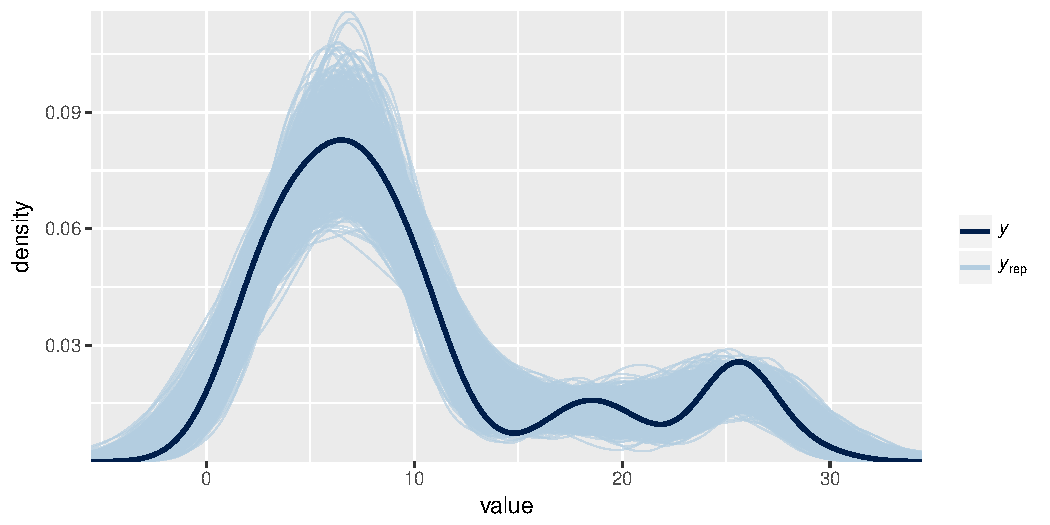
\includegraphics[width=\maxwidth]{figure/datfbm_stan1_res-1} 

}




{\centering \includegraphics[width=\maxwidth]{figure/datfbm_stan1_res-2} 

}



\end{knitrout}

It's also possible to estimate the Hurst coefficient using MCMC. We can then compare the results of Bayesian estimation versus MLE.



\begin{knitrout}
\definecolor{shadecolor}{rgb}{1, 1, 1}\color{fgcolor}\begin{kframe}
\begin{verbatim}
##         lambda       psi     Hurst       MSE
## MLE   5.886029 0.3482860 0.5000000 0.4492881
##       5.825773 0.3515937 0.4643100 0.4782912
## Bayes 6.141937 0.3547621 0.5000000 0.4459796
##       6.471260 0.3733738 0.4749538 0.4816747
\end{verbatim}
\end{kframe}
\end{knitrout}

\section{A data example}

The Tecator data set. How long does it take to use \code{iprior} package? Get same results? Which is better?



\begin{knitrout}
\definecolor{shadecolor}{rgb}{1, 1, 1}\color{fgcolor}\begin{kframe}
\begin{alltt}
\hlstd{mod1.stan} \hlkwb{<-} \hlstr{"
  data \{
    int<lower=0> n; // number of data
    int<lower=0> m; // number of prediction points
    vector[n] y; // data y
    matrix[n,n] H; // the kernel matrix
    matrix[m,n] Hpred; // the kernel matrix for prediction
  \}
  parameters \{
    real alpha;
    real<lower=0> psi;
    real<lower=0> lambda;
  \}
  transformed parameters \{
    cov_matrix[n] Vy;
    Vy = psi * (lambda * H) * (lambda * H) + diag_matrix(rep_vector(1 / psi, n));
  \}
  model \{
    target += multi_normal_lpdf(y | rep_vector(alpha, n), Vy);
    target += cauchy_lpdf(lambda | 0, 10);
  \}
  generated quantities \{
    vector[n] w;
    matrix[n,n] Vw;
    vector[m] yhat;
    vector[m] mu;
    Vw = inverse(Vy);
    w = multi_normal_rng(psi * lambda * H * (Vw * (y - alpha)), Vw);
    mu = alpha + lambda * Hpred * w;
    for (i in 1:m)
      yhat[i] = normal_rng(mu[i], 1 / sqrt(psi));
  \}
"}
\hlstd{m} \hlkwb{<-} \hlkwd{stan_model}\hlstd{(}\hlkwc{model_code} \hlstd{= mod1.stan)}
\hlstd{dat} \hlkwb{<-} \hlkwd{list}\hlstd{(}\hlkwc{y} \hlstd{= mod1}\hlopt{$}\hlstd{Y,} \hlkwc{H} \hlstd{= mod1}\hlopt{$}\hlstd{Hl[[}\hlnum{1}\hlstd{]],} \hlkwc{Hpred} \hlstd{=} \hlkwd{fnH2}\hlstd{(mod1}\hlopt{$}\hlstd{x[[}\hlnum{1}\hlstd{]], absorpTest),}
            \hlkwc{n} \hlstd{= mod1}\hlopt{$}\hlstd{n,} \hlkwc{m} \hlstd{=} \hlkwd{length}\hlstd{(fatTest))}
\end{alltt}
\end{kframe}
\end{knitrout}
\begin{knitrout}
\definecolor{shadecolor}{rgb}{1, 1, 1}\color{fgcolor}\begin{kframe}
\begin{alltt}
\hlstd{mod1.stan.fit} \hlkwb{<-} \hlkwd{sampling}\hlstd{(m,} \hlkwc{data} \hlstd{= dat,} \hlkwc{iter} \hlstd{=} \hlnum{2000}\hlstd{,} \hlkwc{chains} \hlstd{=} \hlnum{4}\hlstd{,} \hlkwc{thin} \hlstd{=} \hlnum{2}\hlstd{,}
                          \hlkwc{pars} \hlstd{=} \hlkwd{c}\hlstd{(}\hlstr{"alpha"}\hlstd{,} \hlstr{"lambda"}\hlstd{,} \hlstr{"psi"}\hlstd{,} \hlstr{"yhat"}\hlstd{))}
\end{alltt}
\end{kframe}
\end{knitrout}
\begin{knitrout}
\definecolor{shadecolor}{rgb}{1, 1, 1}\color{fgcolor}\begin{kframe}
\begin{alltt}
\hlcom{# Diagnostics}
\hlcom{# fit.ggs <- ggs(stan2coda(mod1.stan.fit)[, c("lambda", "psi")])}
\hlcom{# ggs_running(fit.ggs)}
\hlcom{# ggs_autocorrelation(fit.ggs)}
\hlcom{# ggs_compare_partial(fit.ggs)}
\hlstd{theta.hat} \hlkwb{<-} \hlkwd{summary}\hlstd{(mod1.stan.fit)}\hlopt{$}\hlstd{summary[,} \hlnum{1}\hlstd{]}
\hlstd{wherey} \hlkwb{<-} \hlkwd{grep}\hlstd{(}\hlstr{"yhat\textbackslash{}\textbackslash{}["}\hlstd{,} \hlkwd{names}\hlstd{(theta.hat))}
\hlstd{fatTestPredicted1B} \hlkwb{<-} \hlstd{theta.hat[wherey]}
\hlstd{RMSE.Train1B} \hlkwb{<-} \hlnum{1} \hlopt{/} \hlkwd{sqrt}\hlstd{(theta.hat[}\hlstr{"psi"}\hlstd{])}
\hlstd{(RMSE.Test1B} \hlkwb{<-} \hlkwd{sqrt}\hlstd{(}\hlkwd{mean}\hlstd{((fatTestPredicted1B} \hlopt{-} \hlstd{fatTest)} \hlopt{^} \hlnum{2}\hlstd{)))}
\end{alltt}
\begin{verbatim}
## [1] 3.247629
\end{verbatim}
\begin{alltt}
\hlcom{# PPC}
\hlkwd{ppc_dens_overlay}\hlstd{(fatTest,} \hlkwd{as.matrix}\hlstd{(mod1.stan.fit)[, wherey])} \hlopt{+}
  \hlstd{ggplot2}\hlopt{::}\hlkwd{theme_gray}\hlstd{()} \hlopt{+}
  \hlkwd{labs}\hlstd{(}\hlkwc{x} \hlstd{=} \hlstr{"value"}\hlstd{,} \hlkwc{y} \hlstd{=} \hlstr{"density"}\hlstd{)} \hlopt{+}
  \hlkwd{theme}\hlstd{(}\hlkwc{legend.text.align} \hlstd{=} \hlnum{0}\hlstd{)}
\end{alltt}
\end{kframe}

{\centering 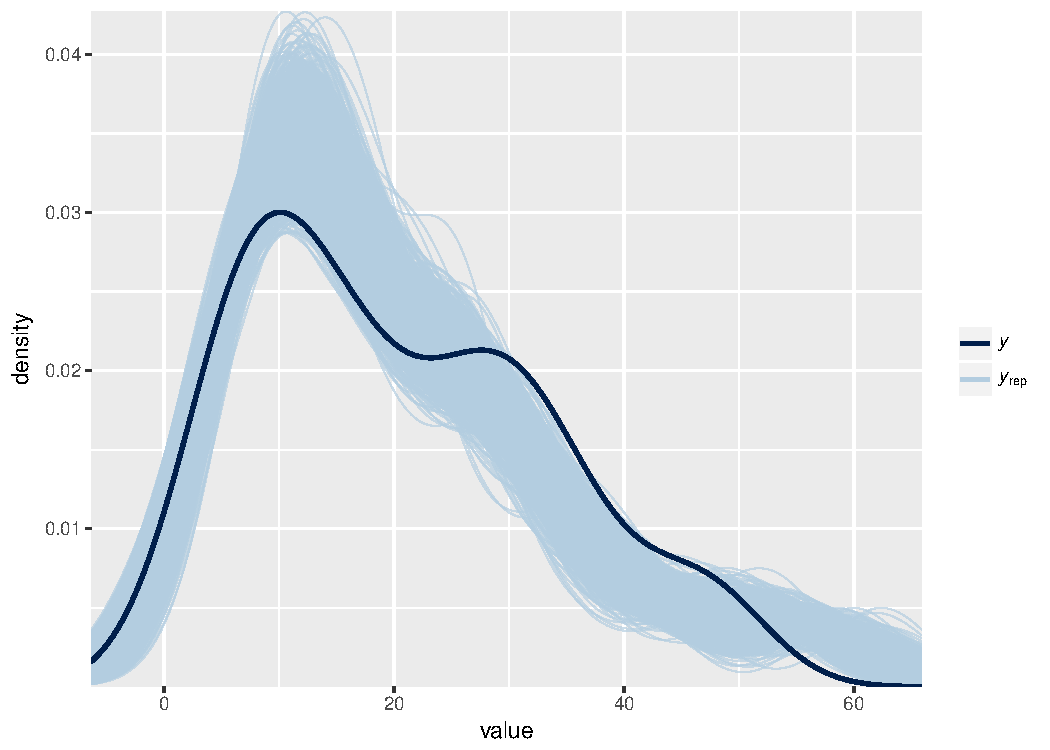
\includegraphics[width=\maxwidth]{figure/tecator_stan1_res-1} 

}



\end{knitrout}

\begin{knitrout}
\definecolor{shadecolor}{rgb}{1, 1, 1}\color{fgcolor}\begin{kframe}
\begin{verbatim}
##         lambda       psi RMSE Test
## MLE   3860.605 0.1234924  3.240386
## Bayes 3751.047 0.1243798  3.247629
\end{verbatim}
\end{kframe}
\end{knitrout}

\section{Discussion}

Summary: competitive performance between Bayes and MLE.

Pro-MLE:

\begin{enumerate}
	\item MLE is much faster.
	\item There are instances where MCMC (even HMC) breaks down. I am referring to the tecator dataset using quadratic/cubic canonical kernel. Bayesian only works for the non-parsimonious case (i.e. separate scale parameter for each kernel).
\end{enumerate}

Pro-Bayes:

\begin{enumerate}
	\item Bayesian inference - parameter described by a posterior density, not just a point estimate.
	\item Able to control informativeness of prior (admittedly, not very relevant for RKHS scale parameters I think).
\end{enumerate}

Implementational issues in HMC:

\begin{enumerate}
	\item Stan throws errors occasionally due to numerical issues. The variance-covariance matrix of $\Vy = \psi \Hlam ^ 2 + \psi^{-1}\bI_n$ can be problematic if $\psi$ is sampled to be extremely small or extremely large. Evident in the Tecator dataset. Possible solutions:
	\begin{enumerate}
		\item Write own code for marginal log-likelihood. This won't be optimised and might run slow.
		\item Stabilise the log-likelihood by working with the Cholesky decomposition of $\Vy$ and the specialised code \verb@multi_normal_cholesky_lpdf@ in \pkg{Stan}.
		\item Stabilise the log-likelihood by performing a spectral decomposition of $\Vy$ to calculate the inverse (precision matrix) and work with the specialised code \verb@multi_normal_prec_lpdf@ in \pkg{Stan}.
	\end{enumerate}
	Neither of these methods completely eliminate the numerical problems, but the problems are not so severe (although they are data dependent). The covariance matrix has potential to be ill-conditioned.
\end{enumerate}

Some notes:

\begin{itemize}
	\item For $\psi$, doesn't really matter what prior is used, this can be estimated quite well. For $\lambda$ however, the choice of prior really affects the results. From a pure Bayesian perspective, this is good, in the sense that your subjective prior matters.
	\item What makes $\lambda$ so hard to estimate?
	\item What is a valid comparison between MLE and Bayes method for I-prior models? Try to use out-of-sample performance.
\end{itemize}

\notodo[Some appendix here?]

%%%%%%%%%%%%%%%%%%%%%%%%%%%%%%%%%%%%%%%%%%%%%%%%%%%%%%%%%%%%%%%%%%%%%%%%
%%% REFERENCES %%%%%%%%%%%%%%%%%%%%%%%%%%%%%%%%%%%%%%%%%%%%%%%%%%%%%%%%%
%%%%%%%%%%%%%%%%%%%%%%%%%%%%%%%%%%%%%%%%%%%%%%%%%%%%%%%%%%%%%%%%%%%%%%%%
%\nocite{*}
%\bibliographystyle{apalike}
%\bibliography{haziq}
%\end{document}

%%%%%%%%%%%%%%%%%%%%%%%%%%%%%%%%%%%%%%%%%%%%%%%%%%%%%%%%%%%%%%%%%%%%%%%%%%%%%%%%
%%% APPENDIX %%%%%%%%%%%%%%%%%%%%%%%%%%%%%%%%%%%%%%%%%%%%%%%%%%%%%%%%%%%%%%%%%%%
%%%%%%%%%%%%%%%%%%%%%%%%%%%%%%%%%%%%%%%%%%%%%%%%%%%%%%%%%%%%%%%%%%%%%%%%%%%%%%%%
%\appendix
%\section{Understanding LDLT decomposition in R}
%\hltodo{Can be removed later on if not relevant}
%
%<<ldlt, cache = TRUE>>=
%library(Matrix)
%(A <- Matrix(c(1, 1, 1, 1, 5, 5, 1, 5, 14), nrow = 3))
%(ch <- chol(A))
%(dd <- diag(ch))
%(L <- t(ch / dd))
%(DD <- dd ^ 2)
%(L %*% diag(DD) %*% t(L))  # get the matrix A = LDL^T back
%@


\end{document}